This section is split into sections describing the verification process for each module and an analysis and discussion of the overall results from the simulation.
\subsection{Verification}
\subsubsection{Fault Injection and Filtering sub modules}\label{sec:verifFaultInjectFilter}
\par Verification for the fault injection and correction modules was completed using the peak signal to noise ratio compared to the reference frame. This is done in the \verb!Verification - 1! and \verb!Verification - 2! blocks as shown in \autoref{fig:verificationBlock}. Data type conversion was completed because the reference frame outputs a single data type and the test frames output a double data type.
\begin{figure}[H]
    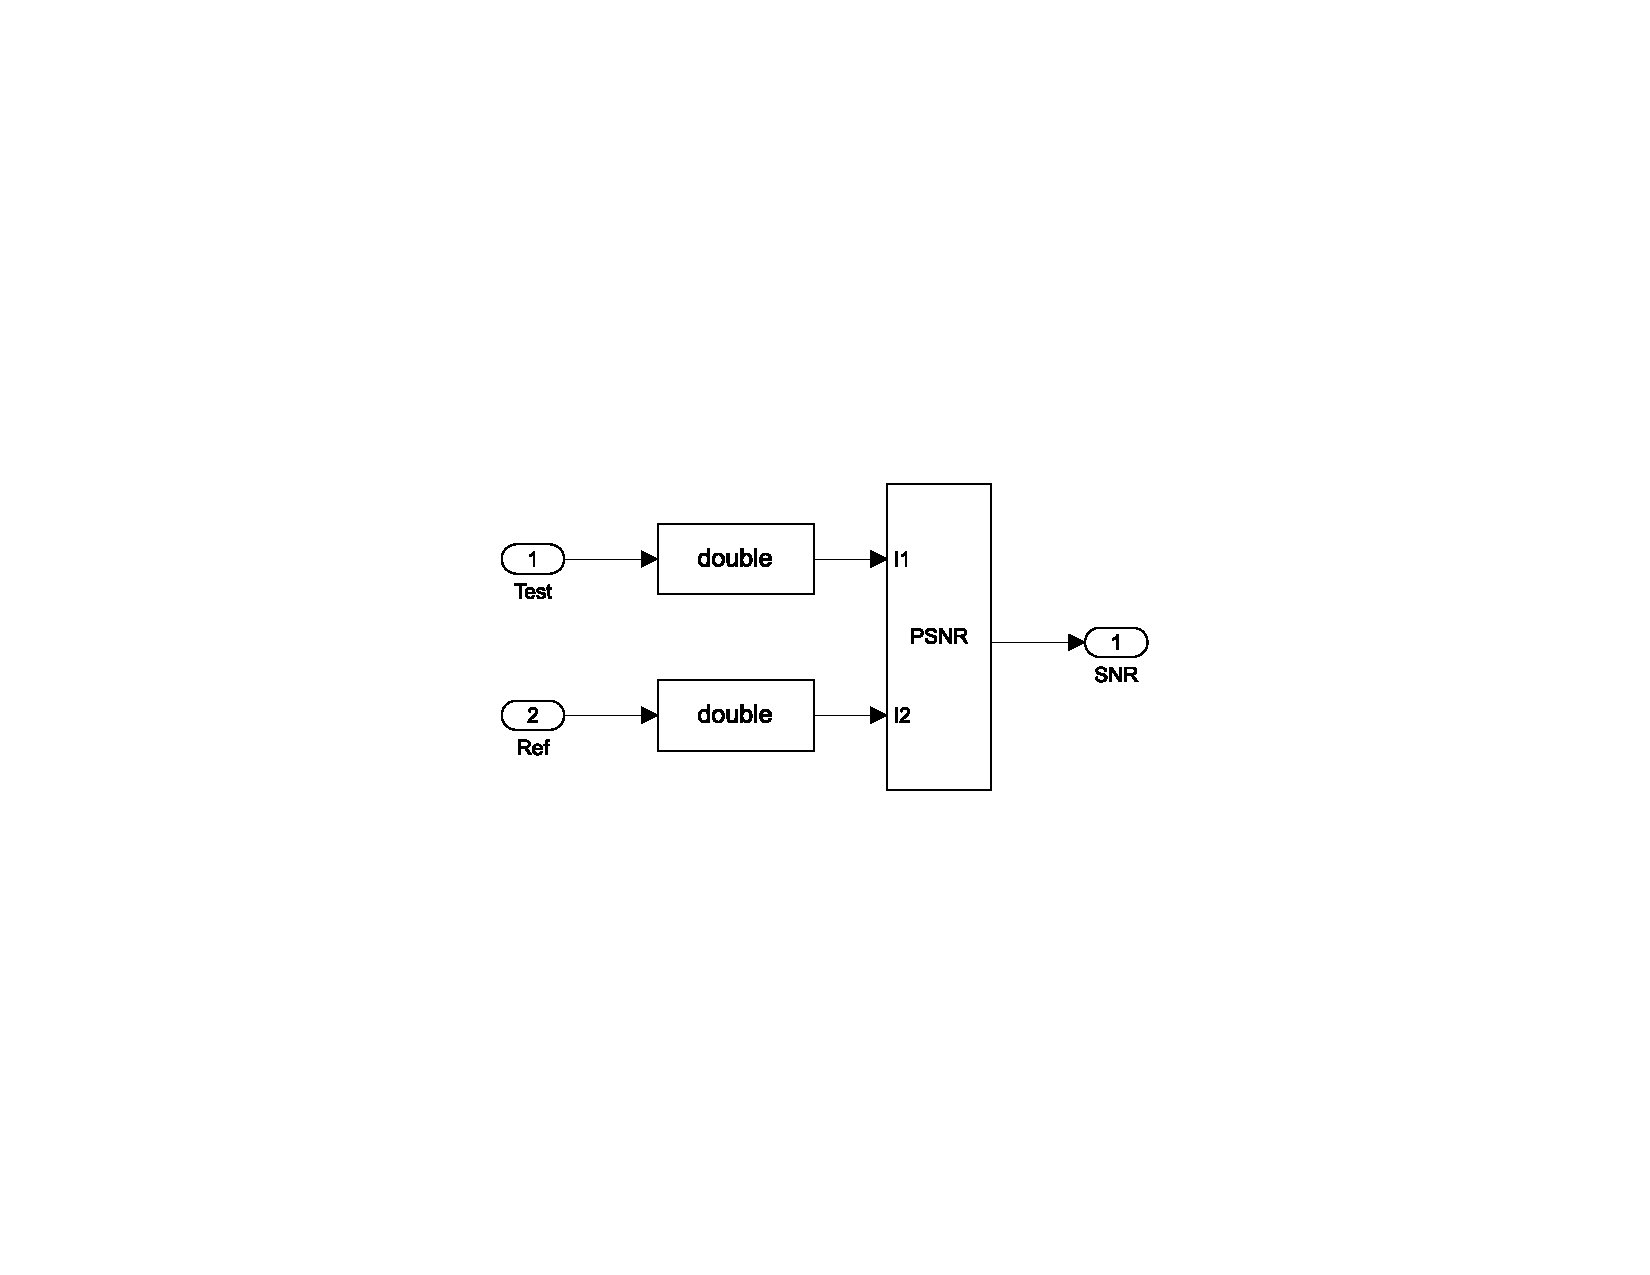
\includegraphics[width=\linewidth]{impl_dsgn_Verification - 1}
    \caption{PSNR Verification}
    \label{fig:verificationBlock}
\end{figure}
\par The PSNR is calculated using the mean-square-error or MSE. The MSE represents the amount the reference image differs from the test image, and PSNR is a measure of the peak error and is calculated by dividing the maximum data type range by the MSE. This document uses floating point, therefore the maximum range is one\cite{mathworks}.
\subsubsection{Permanent Fault Identification sub module}\label{sec:permFaultID}
\par Verification for the noise identification module was conducted differently than the last two. Noise Identification Verification is done by comparing the current frame to the previous frame. The percent difference is captured and overlaid onto the output video as shown in \autoref{fig:noiseIDVer}. A one unit delay block is fed as the \verb!Test! input of this block.
\begin{figure}[H]
    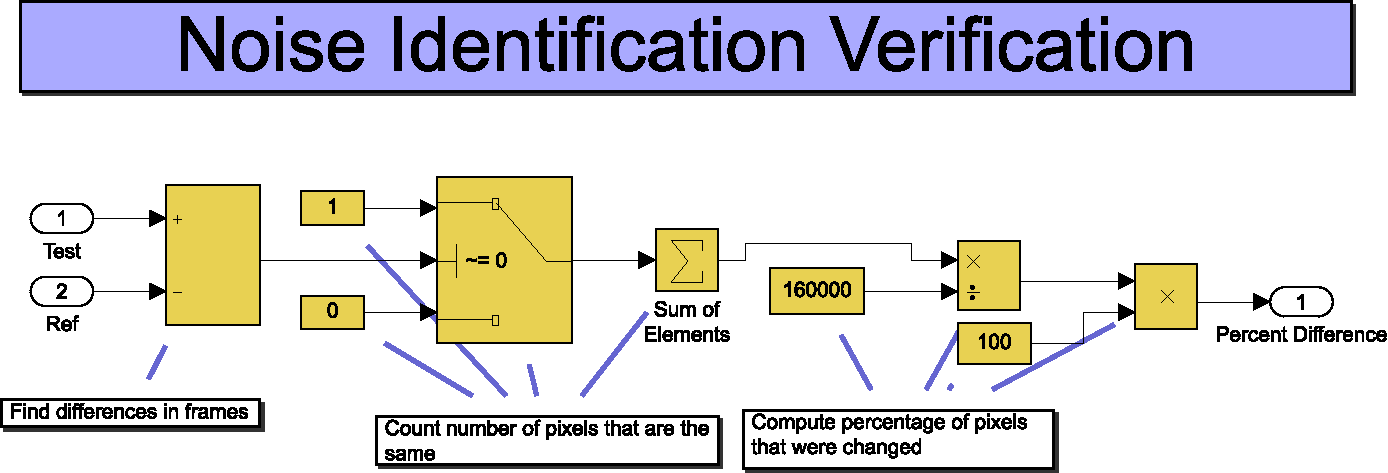
\includegraphics[width=\linewidth]{impl_dsgn_Noise Identification Verification}
    \caption{Noise Identification Verification}
    \label{fig:noiseIDVer}
\end{figure}

\subsection{Analysis}
Analysis can be completed by looking at both numerical data and imagery.
Video recordings for each major output can be downloaded at the following URLs:
\begin{enumerate}\label{list:urlList}
    \item \hyperlink{https://github.com/dgaiero/cpe-446-final-paper/blob/master/design/video-output/compressed/reference.m4v}{Reference Video}
    \item \hyperlink{https://github.com/dgaiero/cpe-446-final-paper/blob/master/design/video-output/compressed/noisyImage.m4v}{Reference with Noise Added Video}
    \item \hyperlink{https://github.com/dgaiero/cpe-446-final-paper/blob/master/design/video-output/compressed/PostNR.m4v}{Post Noise Reduction Video}
    \item \hyperlink{https://github.com/dgaiero/cpe-446-final-paper/blob/master/design/video-output/compressed/noiseIdentification.m4v}{Noise Identification Video}
\end{enumerate}
These URLs link to the latest video stored on the version control management system. They may display a slightly different image than is presented in this paper.
\subsubsection{Noise injection and filtering sub modules}
\par The average PSNR value for the noise generation block is 21.7dB and the average PSNR of the noise filtering block is 66.9dB. For reference, the typical PSNR value for 16-bit lossy image  compression is between 60 to 80dB\cite{welstead_1999}. As expected, the PSNR value for post noise filtering is much higher than the noise generation PSNR. This value is on-par with lossy image compression, which will provide virtually no difference to the viewer. Compared to using just a median filter, this result is marginally superior with a 24.7\% difference (52.2dB for just the median filter versus 66.9dB for the modified median filter). However, by visual inspection, the modified filter is far superior.
\begin{figure}[H]
    \subfloat[Reference Frame 40\label{fig:ref40a}]{%
       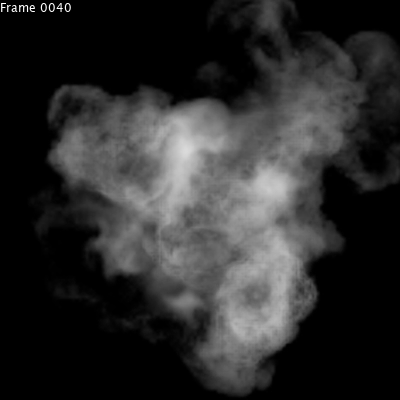
\includegraphics[width=0.45\linewidth]{reference-0040}}
    \hfill
     \subfloat[Noise Reduction Frame 40\label{fig:postNR40a}]{%
        \includegraphics[width=0.45\linewidth]{postNR-0040}}
    \caption{(a), (b) Shown are both reference frame 40 and noise filtering frame 40 showing the results of the modified median filter.}
    \label{fig:ref-postNR40}
\end{figure}
\par Notice how both \autoref{fig:ref40a} and \autoref{fig:postNR40a} are almost visually indistinguishable. Only areas of the image identified as noise use the median filter to reduce noise and it is assumed that all other areas are noise free. For further observation, the reader is encouraged to view the linked videos as identified in the \hyperref[list:urlList]{list} above.
\par The noise identification module outputs a matrix identifying all locations where a permanent fault is located in the input array. This data is then overlaid on top of the noise injected frame.
\begin{figure}[H]
    \subfloat[Permanent Fault Injected Image Frame 65\label{fig:noisyImage65}]{%
       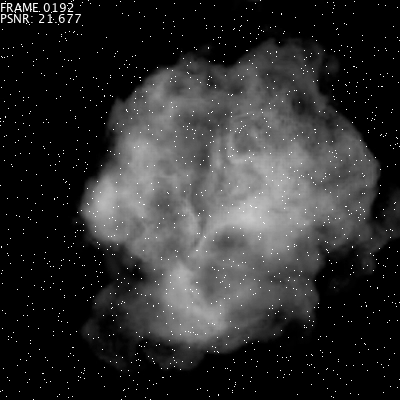
\includegraphics[width=0.45\linewidth]{noisyImage-0065}}
    \hfill
     \subfloat[Permanent Fault Identified Image Frame 65\label{fig:noiseID65}]{%
        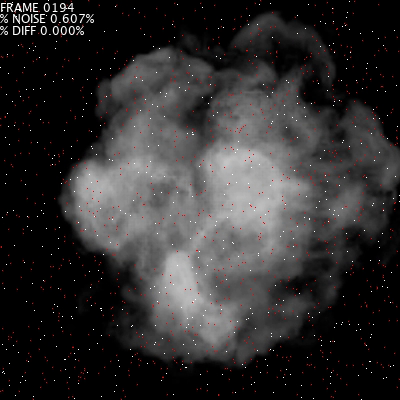
\includegraphics[width=0.45\linewidth]{noiseIdentification-0065}}
    \\
     \subfloat[Permanent Fault Identified Image Frame 75\label{fig:noiseID75}]{%
        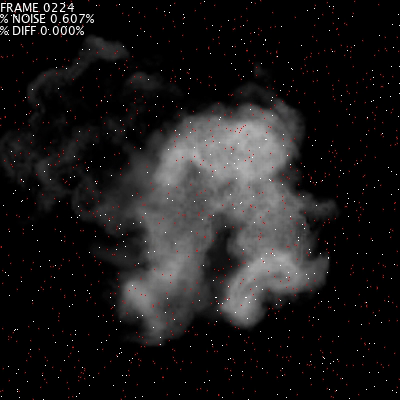
\includegraphics[width=0.45\linewidth]{noiseIdentification-0075}}
    \hfill
     \subfloat[Permanent Fault Identified Image Frame 100\label{fig:noiseID100}]{%
        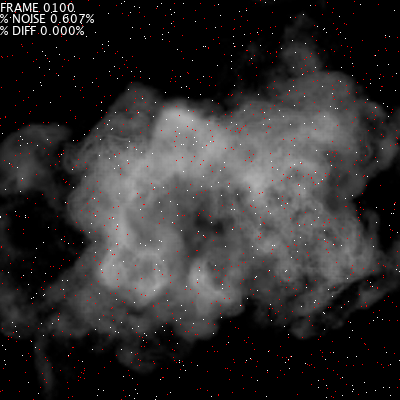
\includegraphics[width=0.45\linewidth]{noiseIdentification-0100}}
    \caption{(a), (b) Shown are both the noise injected frame 65 and permanent fault identification frame 65 showing the effectiveness of the noise identification. (c), (d) show the progression of permanent fault identification throughout the video playback.}
    \label{fig:noisy-ID65}
\end{figure}
\par Since it takes 64 frames to identify noise, the first identified noise will only be output on frame 65, therefore \autoref{fig:noisyImage65} and \autoref{fig:noiseID65} are displaying frame 65. Identified permanent faults are colored red in \autoref{fig:noiseID65} for real-time identification. The percentage of the frame that contains permanent faults is identified in the upper left-hand corner of the frame. Notice how the identified permanent faults do not change between \autoref{fig:noiseID65}, \autoref{fig:noiseID75}, and \autoref{fig:noiseID100}. Additionally, verification information can be read in the upper-left corner. In \autoref{fig:noiseID65} the percent difference is identified as 0.607\%. In \autoref{fig:noiseID75} and \autoref{fig:noiseID100} the percent difference is identified as 0.000\%. This is to be expected, since once the noise is identified, there will be a difference between the previous frame (reference \autoref{sec:permFaultID} for more information on verification of this sub module), and the current frame. However, once these faults are identified, there should be no difference between previous frames. Again, this is outlined in \autoref{fig:noiseID75} and \autoref{fig:noiseID100}. Playback of the video listed in this \hyperref[list:urlList]{list} can also prove this information.
\par Since the seed for the permanent fault injection module is fixed, analysis was done in MATLAB\textregisteredmark\ to determine the accuracy of the SIMULINK\textregisteredmark\ simulation. The MATLAB\textregisteredmark\ yielded the same permanent fault percentage identified in the SIMULINK\textregisteredmark\ model.